\documentclass[a4paper]{article}
\usepackage[left=2cm, right=2cm, top=0.8in, bottom=1.0in]{geometry}
\usepackage{fontspec}
\usepackage{xeCJK}
\usepackage{indentfirst}
\usepackage{setspace}
\usepackage{paralist} 
\usepackage{fancyhdr}
\usepackage[ruled, linesnumbered]{algorithm2e}
\usepackage{setspace}
\usepackage{hyperref}
\usepackage{amsmath}
\usepackage{graphicx}
\usepackage{listings,xcolor}
\usepackage{inconsolata}
\usepackage{tikz,forest}
\usepackage{cite}
\usepackage{booktabs}
\definecolor{mygreen}{rgb}{0,0.6,0}  
\definecolor{mygray}{rgb}{0.5,0.5,0.5}  
\definecolor{mymauve}{rgb}{0.58,0,0.82}  
\pagestyle{fancy}
\fancyhf{}
\fancyhead[L]{数值分析期末实践报告 \quad 郭宇祺} %页眉
\fancyfoot[C]{\thepage}
\let\itemize\compactitem
\let\enditemize\endcompactitem
\let\enumerate\compactenum
\let\endenumerate\endcompactenum
\let\description\compactdesc
\let\enddescription\endcompactdesc
\setstretch{1.35} 
\setlength{\parindent}{2em} 
\setmainfont{Times New Roman}
\setCJKmainfont[BoldFont={黑体}, ItalicFont={楷体}]{宋体}
\setCJKsansfont{黑体}
\setCJKmonofont{仿宋}
\setmonofont{Consolas}
\renewcommand{\lstlistingname}{Lst.}


\lstset{ %  
  backgroundcolor=\color{white},   % choose the background color; you must add \usepackage{color} or \usepackage{xcolor}  
  basicstyle=\footnotesize\ttfamily,        % the size of the fonts that are used for the code  
  breakatwhitespace=true,         % sets if automatic breaks should only happen at whitespace  
  breaklines=true,                 % sets automatic line breaking  
  captionpos=bl,                    % sets the caption-position to bottom  
  commentstyle=\color{mygreen},    % comment style  
  escapeinside={\%*}{*)},          % if you want to add LaTeX within your code  
  extendedchars=true,              % lets you use non-ASCII characters; for 8-bits encodings only, does not work with UTF-8  
  frame=single,                    % adds a frame around the code  
  keepspaces=true,                 % keeps spaces in text, useful for keeping indentation of code (possibly needs columns=flexible)  
  keywordstyle=\color{blue},       % keyword style  
  numbers=left,                    % where to put the line-numbers; possible values are (none, left, right)  
  numbersep=5pt,                   % how far the line-numbers are from the code  
  numberstyle=\tiny\color{mygray}, % the style that is used for the line-numbers  
  rulecolor=\color{black},         % if not set, the frame-color may be changed on line-breaks within not-black text (e.g. comments (green here))  
  showspaces=false,                % show spaces everywhere adding particular underscores; it overrides 'showstringspaces'  
  showstringspaces=false,          % underline spaces within strings only  
  showtabs=false,                  % show tabs within strings adding particular underscores  
  stepnumber=1,                    % the step between two line-numbers. If it's 1, each line will be numbered  
  stringstyle=\color{orange},     % string literal style  
  tabsize=2,                       % sets default tabsize to 2 spaces  
}  

\begin{document} 
\title{数值分析期末实践报告}
\author{郭宇祺}
\date{}
\maketitle
\normalsize
\section{出勤说明}
本人全勤。

\section{LAPACK分析}
\subsection{线性方程组求解函数分析}
对于线性方程组$Ax=b$,LAPACK使用LU分解(等价于高斯消元法)进行求解,涉及的函数包括以下几种,其中xx用于指定输入矩阵的类型,包括稠密矩阵(ge),带状阵(gb)和三对角阵(gt):
\begin{itemize}
  \item \emph{\_xxtrf}: 使用普通的LU分解求解线性方程组。稠密矩阵版本(\emph{\_getrf})和带状阵版本(\emph{\_gbtrf})采用了矩阵分块的性能优化手段,三对角阵版本(\emph{\_gttrf})没有采用特殊的性能优化手段。
  \item \emph{\_xxtrs}: 使用普通的LU分解求解线性方程组。使用\emph{\_xxtrf}作为底层实现,但是与\emph{\_xxtrf}不同之处在于,该函数要求系数矩阵$A$是一个方阵,而\emph{\_xxtrf}没有此要求。与\emph{\_xxtrf}类似,稠密矩阵版本(\emph{\_getrs})和带状阵版本(\emph{\_gbtrs})采用了矩阵分块的性能优化手段,三对角阵版本(\emph{\_gttrs})没有采用特殊的性能优化手段。
  \item \emph{\_xxrfs}: 此算法执行优化迭代,修正解以减少误差并估计(解的)误差的界。三个版本的函数都没有采用特殊的性能优化手段。
\end{itemize}

\subsection{对称特征值问题求解函数分析}

假设$A$是待求特征值的实对称矩阵(厄米特矩阵同理,此处略去),在LAPACK中,首先通过函数\emph{\_sytrd}(稠密存储矩阵)、\emph{\_sptrd}(块状存储矩阵)或\emph{\_sbtrd}(带状存储矩阵)将矩阵$A$归约为实三对角阵$T$,即做分解$A=QTQ^T$。随后对$T$求解特征值问题,即求$T=S\Lambda S^T$,则$\Lambda$的对角元就是$A$的特征值,且$Z=QS$的列向量就是对应的特征向量。函数\emph{\_orgtr}用来显式地计算$Q$。这个函数需要在调用函数\emph{\_steqr}之前被调用,以便计算$A$的特征向量。函数\emph{\_ormtr}用来在不显式计算出$Q$的前提下,计算$Q$左乘另一个矩阵的结果。这个函数可以用来将函数\emph{\_stein}返回的$T$的特征向量重新转变为$A$的特征向量。

用来对矩阵$T$求解特征值问题的函数包括以下几种:
\begin{itemize}
  \item \emph{\_steqr}: 使用隐式提升的QR算法完成计算。它会自动在QR与QL算法中进行切换,以便更高效地处理graded matrices。采用的性能优化方法是矩阵分块。
  \item \emph{\_sterf}: 使用一种无开平方运算的QR算法完成计算。与\emph{\_steqr}一样会自动在QR与QL算法中自动切换。采用的性能优化方法是矩阵分块。
  \item \emph{\_stedc}: 使用一种由Cuppen提出的分治算法进行计算。相比\emph{\_steqr},在大矩阵上其运行速度可能快数倍,但是需要更大的内存开销($2n^2$或$3n^2$)。没有采用特殊的优化手段。
  \item \emph{\_stegr}: 使用relatively robust representation (RRR)算法完成计算。除了在某些特定例子上,该函数的运行速度比其他所有函数都快,并且使用的内存开销也最小。采用的性能优化方法是矩阵分块。
  \item \emph{\_pteqr}: 此函数仅用于计算对称正定的三对角阵的特征值问题。它使用了一种由Cholesky分解和双对角QR迭代算法组合而成的算法。该函数的计算结果比其他所有函数(除了\emph{\_stegr})都要准确。没有采用特殊的优化手段。
  \item \emph{\_stebz}: 此函数使用二分法计算全部或部分特征值。它可以通过降低对结果的精确度要求来获得更快的运行速度。采用的性能优化方法是分块。
  \item \emph{\_stein}: 此函数用来在给定准确的特征值的前提下通过反向迭代计算部分或全部的特征向量。没有采用特殊的优化手段。
\end{itemize}

\section{最小二乘法曲线拟合}
\subsection{算法简介}
给定观测数据$(x_i, y_i), i=1, 2, \dots m$,欲通过最小二乘法求解其N次多项式曲线$f(x)=a_0+a_1x+a_2x^2+\dots+a_nx^n$的拟合参数,可通过求解以下线性方程组获得:

\begin{equation*}
  A^TA
  \begin{bmatrix}
    a_0 \\
    a_1 \\
    \vdots \\
    a_n
  \end{bmatrix}
  =A^T
  \begin{bmatrix}
    y_1 \\
    y_2 \\
    \vdots \\
    y_m
  \end{bmatrix}
\end{equation*}

其中矩阵$A$是如下所示的范德蒙矩阵:

\begin{equation*}
  A=
  \begin{bmatrix}
    1 & x_1 & x_1^2 & x_1^3 & \cdots & x_1^n \\
    1 & x_2 & x_2^2 & x_2^4 & \cdots & x_2^n \\
    1 & x_3 & x_3^2 & x_3^3 & \cdots & x_3^n \\
    \vdots & \vdots & \vdots & \vdots & & \vdots \\
    1 & x_m & x_m^2 &x_m^3 & \cdots & x_m^n
  \end{bmatrix}
\end{equation*}

\subsection{具体实现及工具说明}
曲线拟合参数计算程序使用C/C++语言编写,运行脚本及绘图脚本使用python语言编写。
C/C++编译器使用Clang/LLVM 12.0,编译标准使用C++17,优化等级指定为O3。在python绘图脚本中,绘图库使用matplotlib.pyplot。实验平台采用Ubuntu 20.04LTS,机器配置为CPU Intel(R) Xeon(R) Platinum 8260 @ 2.40GHz(48核心96线程),内存大小512GB。

实验中,分别使用三种数学库组合作为后端进行最小二乘计算,他们是:
\begin{itemize}
  \item CBLAS-v3.11.0 + LAPACKE-v3.11.0 
  \item GotoBLAS2-v1.13 + clapack-v3.10.3-8ubuntu7
  \item ATLAS-v3.10.3-8ubuntu7 + clapack-v3.10.3-8ubuntu7
\end{itemize}

以下简要说明工具的编译及使用方法。

首先使用以下命令编译曲线拟合参数计算程序:
\begin{lstlisting}
  mkdir build
  cd build
  cmake ..
  make   
\end{lstlisting}
在执行cmake指令时需要额外添加编译选项-DBUILD\_LAPACK\_FROM\_SRC=ON,-DBUILD\_GOTO2=ON或-DBUILD\_ATLAS=ON,以指定使用的后端数学库。否则会遇到编译报错。完成编译后,生成的二进制曲线拟合参数计算程序main会生成在bin文件夹下。

main程序可以完成随机数据生成以及多项式曲线拟合参数计算的工作,其接受以下参数:
\begin{itemize}
  \item -M,指定随机生成的观察数据的个数(必需)
  \item -k,指定参数k(必需)
  \item -N,指定需要拟合的曲线的度数(必需)
  \item -r,指定原始观察数据的输出文件夹(非必需,默认生成在当前路径下)
  \item -f,指定曲线拟合参数的输出文件夹(非必需,默认生成在当前路径下)
\end{itemize}

可以使用自动运行脚本generate.py完成曲线拟合参数计算程序的运行以及后续的绘图工作,命令如下:
\begin{lstlisting}
  python3 ./generate.py
\end{lstlisting}
generate.py中已经定义了一系列待测试的(M, k, N)参数,如有需要可自行修改。绘制得到的图片存储在figures文件夹下。

\subsection{测试结果}
\subsubsection{拟合效果展示及对比}
由于测试数据较多(全部测试数据详见表\ref{tlb:perf}),因此本小节中仅展示部分具有代表意义的拟合效果曲线图。实验所涉及的全部拟合效果曲线图可在文件夹figures下找到。

\begin{figure}[tbp]
  \centering
  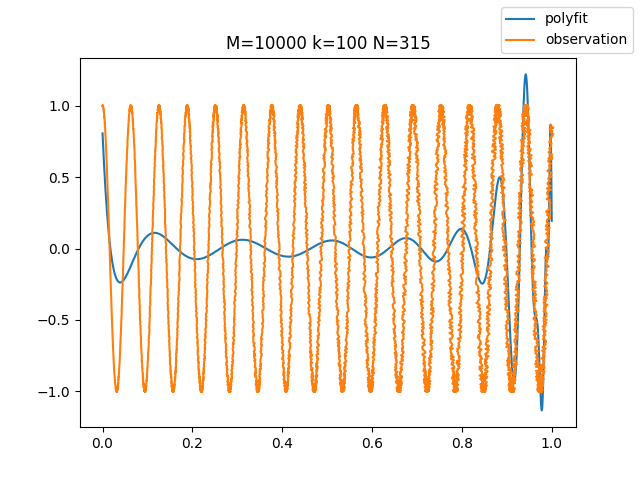
\includegraphics[width=0.5\textwidth]{figures/lapack/figure0_M_10000_k_100_N_315.png}
  \caption{M=10000, k=100, N=315, CBLAS}
  \label{fig:exp1}
\end{figure}

\begin{figure}[tbp]
  \centering
  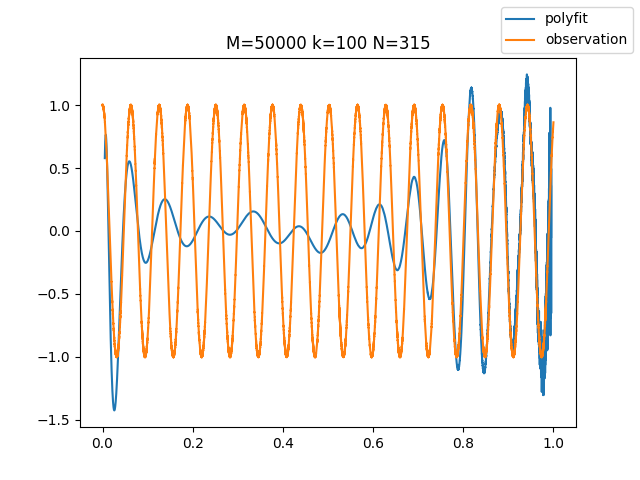
\includegraphics[width=0.5\textwidth]{figures/lapack/figure1_M_50000_k_100_N_315.png}
  \caption{M=50000, k=100, N=315, CBLAS}
  \label{fig:exp2}
\end{figure}

\begin{figure}[tbp]
  \centering
  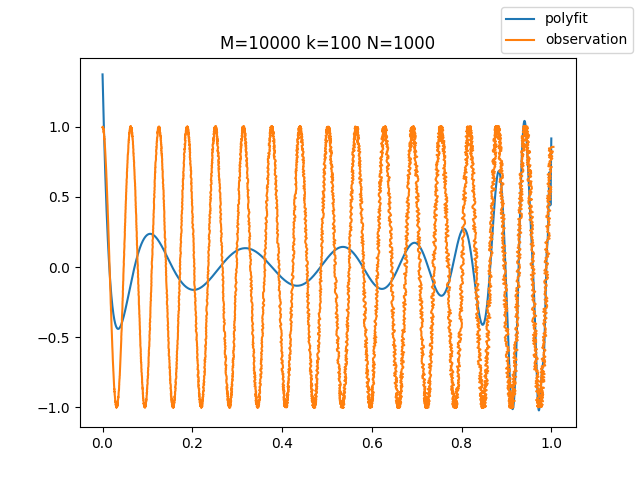
\includegraphics[width=0.5\textwidth]{figures/lapack/figure5_M_10000_k_100_N_1000.png}
  \caption{M=10000, k=100, N=1000, CBLAS}
  \label{fig:exp3}
\end{figure}

\begin{figure}[tbp]
  \centering
  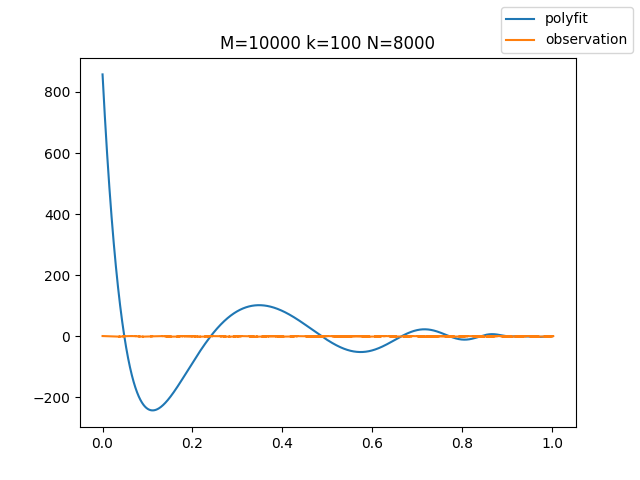
\includegraphics[width=0.5\textwidth]{figures/lapack/figure8_M_10000_k_100_N_8000.png}
  \caption{M=10000, k=100, N=8000, CBLAS}
  \label{fig:exp4}
\end{figure}

\begin{figure}[tbp]
  \centering
  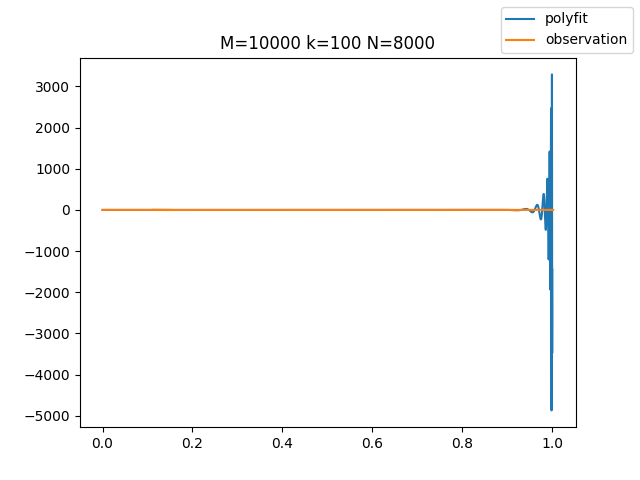
\includegraphics[width=0.5\textwidth]{figures/atlas/figure7_M_10000_k_100_N_8000.png}
  \caption{M=10000, k=100, N=8000, ATLAS}
  \label{fig:exp5}
\end{figure}

\begin{figure}[tbp]
  \centering
  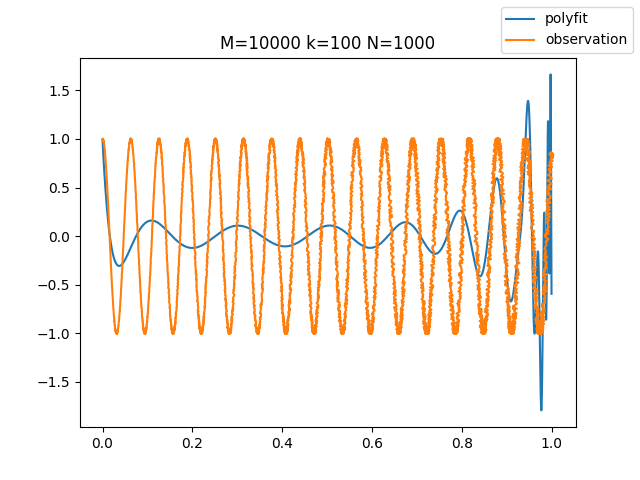
\includegraphics[width=0.5\textwidth]{figures/atlas/figure4_M_10000_k_100_N_1000.png}
  \caption{M=10000, k=100, N=1000, ATLAS}
  \label{fig:atlas}
\end{figure}


当参数k取较小值(以k=100为例),且多项式度数$N$在$\pi k$附近取值时,在$x \in [0.8, 1.0]$区间上以及零点附近,拟合所得多项式曲线能够较好地贴合原始曲线,如图\ref{fig:exp1}所示,其中橙色曲线为原始观测数据,蓝色曲线为拟合所得的多项式曲线;但是在$x \in (0, 0.8)$区间上,由于双精度数据结构精度所限,高次项信息几乎完全丢失,因此拟合效果不够理想,仅能够勉强拟合出原始曲线起伏的变化趋势。增大观测数据的数量$M$对曲线拟合几乎没有帮助,如图\ref{fig:exp2}所示。增大待拟合多项式的度数$N$能够在一定程度上取得更好的效果,拟合曲线在$x \in (0, 0.8)$区间上的起伏会变得更大从而更贴近原始曲线,但仍然无法捕获原始曲线中存在的高频信息,如图\ref{fig:exp3}所示。并且,当$N$取值过大时,拟合曲线在靠近0点附近(CBLAS)或靠近1点(GotoBLAS2和ATLAS)附近可能会面临取值爆炸的问题,如图\ref{fig:exp4}和\ref{fig:exp5}所示。三种数学库组合在处理这些参数时表现差异不大,主要区别在于CBLAS + LAPACKE组合拟合得到的曲线较为光滑,而其他两种数学库组合得到的拟合曲线可能出现较多的毛刺,如图\ref{fig:atlas}所示。此种差异可能是由于所使用的lapack库不同所导致的。由于GotoBLAS2和ATLAS均与LAPACKE存在头文件冲突,因此在实验中使用ATLAS自带的lapack库clapack作为替代。

\begin{figure}[tbp]
  \centering
  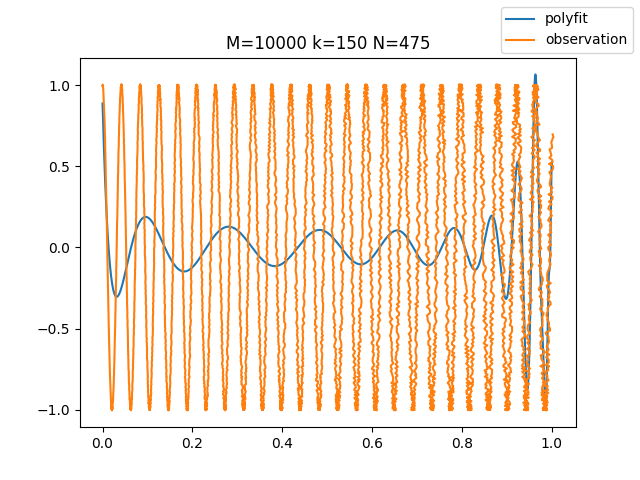
\includegraphics[width=0.5\textwidth]{figures/lapack/figure18_M_10000_k_150_N_475.png}
  \caption{M=10000, k=150, N=475, CBLAS}
  \label{fig:exp6}
\end{figure}

\begin{figure}[tbp]
  \centering
  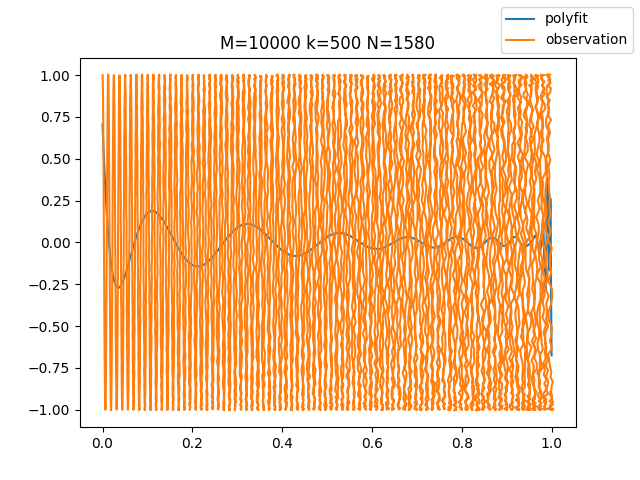
\includegraphics[width=0.5\textwidth]{figures/lapack/figure35_M_10000_k_500_N_1580.png}
  \caption{M=10000, k=500, N=1580, CBLAS}
  \label{fig:exp7}
\end{figure}

\begin{figure}[tbp]
  \centering
  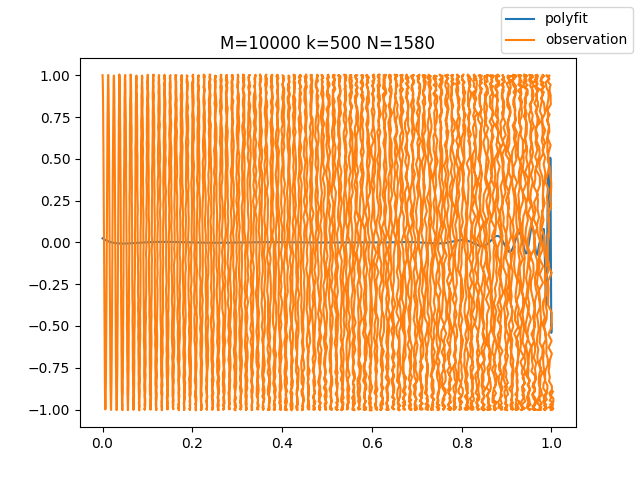
\includegraphics[width=0.5\textwidth]{figures/atlas/figure31_M_10000_k_500_N_1580.png}
  \caption{M=10000, k=500, N=1580, ATLAS}
  \label{fig:exp8}
\end{figure}

随着参数k的增大,由于随机扰动的存在,拟合效果会逐渐变差,只有在非常靠近1点的很小区间内拟合曲线能够较好地贴合原始曲线,在其他区间只能非常粗略地捕获到原始曲线的起伏信息,如图\ref{fig:exp6}和\ref{fig:exp7}所示。在处理这些参数时,使用LAPACKE的CBLAS的效果明显好于使用clapack的GotoBLAS2和ATLAS:当参数k取一个较大值500时,前者拟合得到的曲线在$x \in (0, 0.8)$区间上仍呈现出了一定的起伏趋势,如图\ref{fig:exp7}所示;而后者在该区间上所得的拟合曲线呈几乎没有起伏的直线,如图\ref{fig:exp8}所示。






\subsubsection{不同数学库拟合效率对比}
表\ref{tlb:perf}展示了三种数学库在各种参数组合下计算曲线拟合参数所需的时间,其中耗时数据的单位为秒。我同时计算了GotoBlas2 + clapack和ATLAS + clapack这两种数学库组合相比于CBLAS + LAPACKE在时间上取得的加速比,相关结果展示在\emph{SpeedUp}列中。由于GotoBLAS2库使用多个线程进行矩阵运算,而CBLAS和ATLAS库均只使用一个线程进行运算,因此,为了使对比更为公平,我在实验中统计GotoBLAS2库所有线程耗时的总和作为其耗时的数据。

从表\ref{tlb:perf}中可以看出,相比于基础的CBLAS + LAPACKE组合,GotoBLAS2 + clapack组合在计算效率上没有取得优势,并且由于管理多个线程引起的额外开销,其在总体耗时上略高于CBLAS + LAPACKE组合(平均计算效率约为CBLAS + LAPACKE组合的0.88倍)。但是其通过引入并行机制,可以大大提高程序的运行效率。在本次实验中,我观察到GotoBLAS2 + clapack组合最多可以使用32个线程进行并行运算,因此相比于CBLAS + LAPACKE组合,GotoBLAS2 + clapack组合在运行效率上的加速比能达到约$0.88\times 32=28.16$,从而实现较好的加速效果。ATLAS + clapack组合则主要通过算法优化来实现运行加速。在与CBLAS + LAPACKE组合同样采用单线程模式运行的前提下,ATLAS + clapack组合相较于CBLAS + LAPACKE组合在运行时间上取得的平均加速比为3.77。因此使用ATLAS + clapack组合在无法并行运算的环境下也能够取得不错的加速效果。



\begin{table}[tbp]
  \centering
  \caption{三种数学库曲线拟合耗时信息统计}
  \begin{tabular}{l|r|rr|rr}
    \toprule
    参数组合(M, k, N) & CBLAS + LAPACKE & GotoBLAS2 + clapack & SpeedUp & ATLAS + clapack & SpeedUp\\
    \midrule
    (10000, 100, 315) & 1.57 & 2.16 & 0.73x & 0.43 & 3.65x \\
    \midrule
    (50000, 100, 315) & 8.30 & 8.62 & 0.92x & 1.99 &  4.17x \\
    \midrule
    (10000, 100, 400) & 2.70 & 3.64 & 0.74x & 0.73 & 3.70x \\
    \midrule
    (10000, 100, 500) & 4.54 & 5.70 & 0.80x & 1.26 & 3.60x \\
    \midrule
    (10000, 100, 1000) & 19.63 & 20.06 & 0.98x  & 5.53 & 3.55x \\
    \midrule
    (10000, 100, 2000) & 81.14 & 88.66 & 0.92x & 22.22 & 3.65x\\
    \midrule
    (10000, 100, 5000) & 535.61 & 649.73 & 0.82x & 139.57 & 3.84x \\
    \midrule
    (10000, 100, 8000) & 1412.61 & 1622.28 & 0.87x & 344.35 & 4.10x \\
    \midrule
    (10000, 120, 380) & 2.39 & 3.21 & 0.74x & 0.65 & 3.68x \\
    \midrule
    (50000, 120, 380) & 12.67 & 13.15 & 0.96x & 3.19 & 3.97x \\
    \midrule
    (10000, 120, 500) & 4.49 & 5.75 & 0.78x &  1.24 & 3.62x \\
    \midrule
    (10000, 120, 800) & 12.47 & 13.96 & 0.89x & 3.43 & 3.64x \\
    \midrule
    (10000, 120, 1000) & 19.53 & 20.33 & 0.96x &  5.34 & 3.66x\\
    \midrule
    (10000, 120, 2000) & 80.70 & 89.69 & 0.90x & 22.11 & 3.65x \\
    \midrule
    (10000, 120, 5000) & 539.62 & 650.14 & 0.83x & 140.34 & 3.85x\\
    \midrule
    (10000, 120, 8000) & 1419.56 & 1624.80 & 0.87x & 341.58 & 4.16x\\
    \midrule
    (10000, 150, 475) & 3.99 & 5.18 & 0.77x  & 1.10 & 3.63x \\
    \midrule
    (50000, 150, 475) & 20.83 & 20.71 & 1.00x & 5.36 & 3.89x \\
    \midrule
    (10000, 150, 500) & 4.48 & 5.76 & 0.78x & 1.24 & 3.61x \\
    \midrule
    (10000, 150, 800) & 12.47 & 13.98 & 0.89x & 3.42 & 3.65x \\
    \midrule
    (10000, 150, 1000) & 19.53 & 20.31 & 0.96x & 5.35 & 3.65x \\
    \midrule
    (10000, 150, 2000) & 80.71 & 88.88 & 0.91x &22.12 & 3.65x \\
    \midrule
    (10000, 150, 5000) & 539.83 & 649.92 & 0.83x &138.86 & 3.89x \\
    \midrule
    (10000, 150, 8000) & 1435.05 & 1625.58 & 0.88x &339.63 & 4.23x \\
    \midrule
    (10000, 200, 630) & 7.51 & 9.09 & 0.83x & 2.07 & 3.63x \\
    \midrule
    (50000, 200, 630) & 38.11 & 36.55 & 1.04x & 10.17 & 3.75x \\
    \midrule
    (10000, 200, 800) & 12.44 & 13.95 & 0.89x & 3.41 & 3.65x \\
    \midrule
    (10000, 200, 1000) & 19.47 & 20.14 & 0.97x & 5.36 & 3.63x \\
    \midrule
    (10000, 200, 2000) & 80.44 & 88.80 & 0.91x &  22.14 & 3.63x \\
    \midrule
    (10000, 200, 5000) & 538.72 & 651.66 & 0.83x & 139.83 & 3.85x \\
    \midrule
    (10000, 200, 8000) & 1428.07 & 1625.10 & 0.88x & 338.92 & 4.21x \\
    \midrule
    (10000, 500, 1580) & 49.48 & 50.61 & 0.98x & 13.48 & 3.67x \\
    \midrule
    (50000, 500, 1580) & 243.95 & 235.18 & 1.04x & 66.93 & 3.67x \\
    \midrule
    (10000, 500, 3000) & 187.54 & 226.16 & 0.83x & 50.89 & 3.68x  \\
    \midrule
    (10000, 500, 5000) & 537.23 & 649.43 & 0.83x & 139.94 & 3.84x \\
    \midrule
    (10000, 500, 8000) & 1425.89 & 1624.83 & 0.88x & 342.92 & 4.16x \\
    \midrule
    (50000, 500, 3000) & 874.40 & 1090.35 & 0.80x & 244.21 & 3.58x\\
    \midrule
    平均值 & - & - & 0.88x & -  & 3.77x \\
    \bottomrule    
  \end{tabular}
  \label{tlb:perf}
\end{table}




\end{document}